\documentclass{article}
\usepackage[margin=1in]{geometry}
\usepackage{graphicx}

\begin{document}
\noindent Consider the current mirror shown below. 

\begin{figure}[h]
    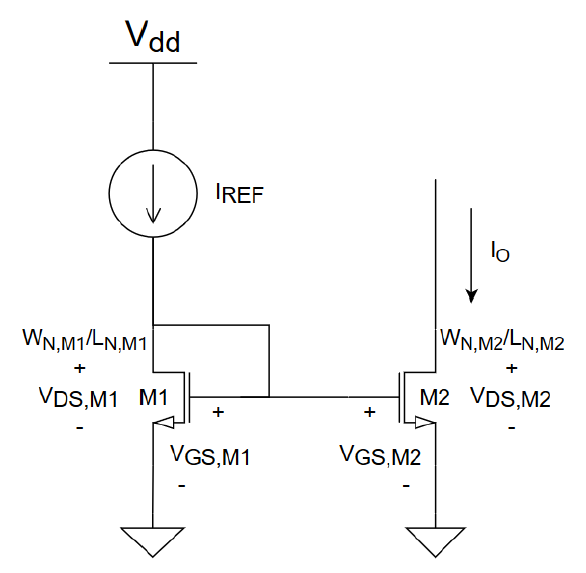
\includegraphics[scale=0.4]{mir}
\end{figure} 

\noindent For any long - channel NMOS, 
$$I_{DS} = \frac{1}{2} \mu_{n} C_{ox} \frac{W}{L} (V_{GS}-V_{TH})^{2} (1+\lambda V_{DS})$$
Solving for $V_{GS}$ in terms of $I_{DS}$, 
\large
$$V_{GS} = \left( \frac{I_{DS}}{\frac{1}{2} \mu_{n} C_{ox} \frac{W}{L} (1+\lambda V_{DS})} \right)^{\frac{1}{2}} + V_{TH}$$
\normalsize 
Notice that $V_{GS,M1} = V_{GS,M2}$. If the transistors have the same mobility $\mu_{n}$, \\gate-oxide
capacitance $C_{ox}$ and threshold voltage $V_{TH}$,

\vspace{10pt}
\noindent since $I_{DS,M1} = I_{REF}$ and $I_{DS,M2} = I_{O}$, 
\large 
$$\frac{I_{REF}}{\frac{W_1}{L_1}(1+\lambda_1 V_{DS,1})} = \frac{I_{O}}{\frac{W_2}{L_2}(1+\lambda_2 V_{DS,2})}$$
\normalsize Finally, 
\large
$$I_{O} = I_{REF} \cdot \frac{\frac{W_2}{L_2}(1+\lambda_2 V_{DS,2})}{\frac{W_1}{L_1}(1+\lambda_1 V_{DS,1})}$$
If both transistors are sized in a way that they have the same lengths, then, 
$$I_{O} = I_{REF} \cdot \frac{W_{2}(1+\lambda V_{DS,2})}{W_{1}(1+\lambda V_{DS,1})}$$

\newpage 

\noindent $A_{v} \geq 25$, $g_{mn} \geq 1mS$.
\vspace{8pt}
\\
\noindent We can start with $r_{on} = r_{op}$ so that $r_{on} \| r_{op} = \frac{1}{2} r_{on}$.
\vspace{8pt}
\\ Thus, $A_{v} = \frac{1}{2} g_{mn} r_{on}$  
\vspace{8pt}
\\ Obtaining $r_{on}$, we get $r_{on} = \frac{2A_v}{g_{mn}} = 50k\Omega = r_{op}$. 

\vspace{20pt}
\noindent Since $r_{on} = 50k\Omega$ and $g_{mn} \geq 1mS$,
\vspace{8pt}
\\ $g_{mn}r_{on} \geq 50$, and the minimum $g_{mn}r_{on} = 50$

\vspace{20pt}
\noindent We know that $A_v = g_{mn}(r_{on}\|r_{op})$
\vspace{8pt}
\\ Thus, $\frac{1}{g_{mn}r_{op}} = \frac{1}{A_v} - \frac{1}{g_{mn}r_{on}}$
\vspace{4pt}
\\ Solving for $r_{op}$ we get $r_{op} = 65.064k\Omega \approx 65k\Omega$

\vspace{20pt}
\Large
\noindent $k_{multiplier} = \frac{1mS}{8uS} = 125$
\normalsize 
\vspace{8pt}
\\ $W_N = 62.5um$, $I_{DN} = 101.7uA$

\vspace{20pt}
\noindent 
We want $I_{DN} = I_{DP} = 101.7uA$
\vspace{8pt}
\Large
\\ $k_{multiplier} = \frac{101.7uA}{1uA} = 101.7$
\vspace{8pt}
\normalsize
\\$W_{P} = 101.7 \cdot 2um = 203.4um$


\vspace{20pt}
\noindent 
Since the biasing transistor has $I_{REF} = 10\mu A$, and we want $I_{DS} = I_{DP} = 101.7\mu A$,
\vspace{8pt}
\\ We design the biasing transistor such that they have the same lengths but their widths follow the 
ratio 
\large 
$$\frac{W_{P}}{W_{REF}} = \frac{101.7\mu}{10\mu} = 10.17$$ 
\normalsize
The biasing transistor should have a width that is $10.17$ times smaller than the width of the active
PMOS load.
\large
$$W_{REF} = \frac{203.4\mu m}{10.17} = 20\mu m$$













\end{document}